\chapter{Keil MCB1700 Hardware Environment}
\label{ch_keil_hardware}
% overview of the board
\section{MCB1700 Board Overview}
The Keil MCB1700 board is populated with {\em NXP LPC1768} Microcontroller. Figure \ref{fig_board_components} shows the important interface and hardware components of the MCB1700 board. 


%MCB1700 Block Diagram
\begin{figure}
\centerline{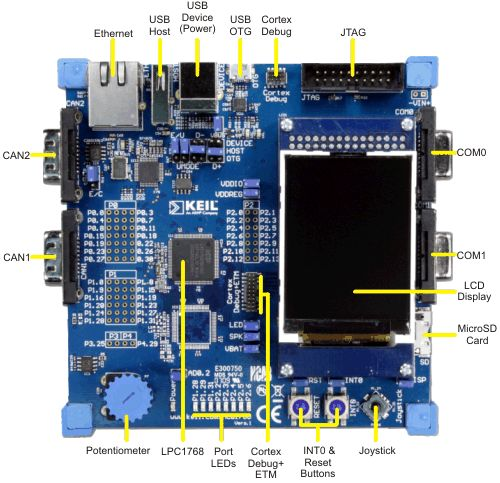
\includegraphics[width=4in]{figure/MCB1700_Board_Components}}
\caption[MCB1700 Board Components] {MCB1700 Board Components \cite{keil.mcb1700.guide}}
\label{fig_board_components}
\end{figure}
Figure \ref{fig_board_block} is the hardware block diagram that helps you to understand the MCB1700 board components. Note that our lab will only use a small subset of the components which include the LPC1768 CPU, COM and Dual RS232. 
\begin{figure}
\centerline{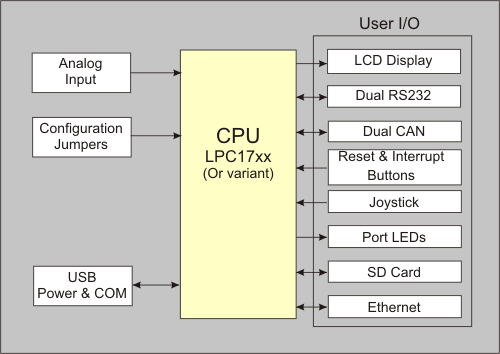
\includegraphics[width=4in]{figure/mcb1700_block_diagram}}
\caption[MCB1700 Board Block Diagram] {MCB1700 Board Block Diagram \cite{keil.mcb1700.guide}}
\label{fig_board_block}
\end{figure}

The LPC1768 is a 32-bit ARM Cortex-M3 microcontroller for embedded applications requiring a high level of integration and low power dissipation. 
The LPC1768 operates at up to an 100 MHz CPU frequency. 
The peripheral complement of LPC1768 includes 512KB of on-chip flash memory, 64KB of on-chip SRAM and a variety of other on-chip peripherals. 
Among the on-chip peripherals, there are system control block, pin connect block, 4 UARTs and 4 general purpose timers, some of which will be used in your RTX  course project.
Figure \ref{fig_lpc1768_block} is the simplified LPC1768 block diagram \cite{nxp.lpc17xx.manual}, where the components to be used in your RTX project are circled with red.  
Note that this manual will only discuss the components that are relevant to the RTX course project. The LPC17xx User Manual is the complete reference for LPC1768 MCU.

% LPC1768 block diagram
\begin{figure}
\centerline{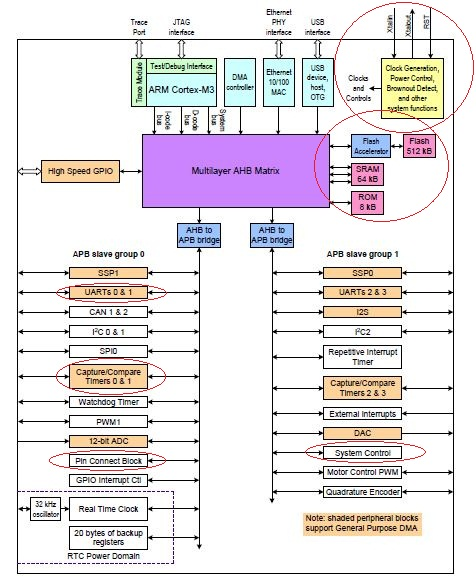
\includegraphics[width=5in]{figure/lpc1768_block_diagram_circled}}
\caption[LPC1768 Block Diagram] {LPC1768 Block Diagram. The circled blocks are the ones that we will use in the lab project.}
\label{fig_lpc1768_block}
\end{figure}


% LPC1768 Core Processor 
\section{Cortex-M3 Processor}
\label{sec_cm3}

The Cortex-M3 processor is the central processing unit (CPU) of the LPC1768 chip.
The processor is a 32-bit microprocessor with a 32-bit data path, a 32-bit register bank, and 32-bit memory interfaces.
Figure \ref{fig_cm3_block} is the simplified block diagram of 
the Cortex-M3 processor \cite{yiu2009definitive}.
%The processor has a Harvard architecture. The separate instruction and data buses share the same memory space 
The processor has private peripherals which are system control block, system timer, NVIC (Nested Vectored Interrupt Controller) and MPU (Memory Protection Unit).
% The MPU programming is not required in the course project.
The processor includes a number of internal debugging components which provides
debugging features such as breakpoints and watchpoints.
%Section \ref{sec_op_mode} discusses the operation mode of the processor. 
%Section \ref{sec_cm3_registers} discusses the Cortex-M3 registers. 

\begin{figure}
\centerline{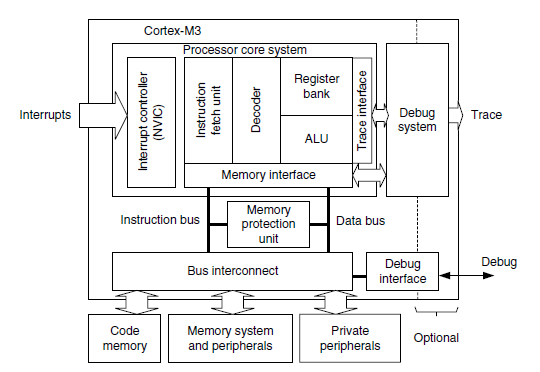
\includegraphics[width=5in]{figure/CortexM3_Processor}}
\caption[Simplified Cortex-M3 Block Diagram] {Simplified Cortex-M3 Block Diagram\cite{yiu2009definitive}}
\label{fig_cm3_block}
\end{figure}

\subsection{Registers}
\label{sec_cm3_registers}
The processor core registers are shown in Figure \ref{fig_cm3_registers}. For detailed description of each register, Chapter $34$ in \cite{nxp.lpc17xx.manual} is the complete reference. 
\begin{figure}[h]
\centerline{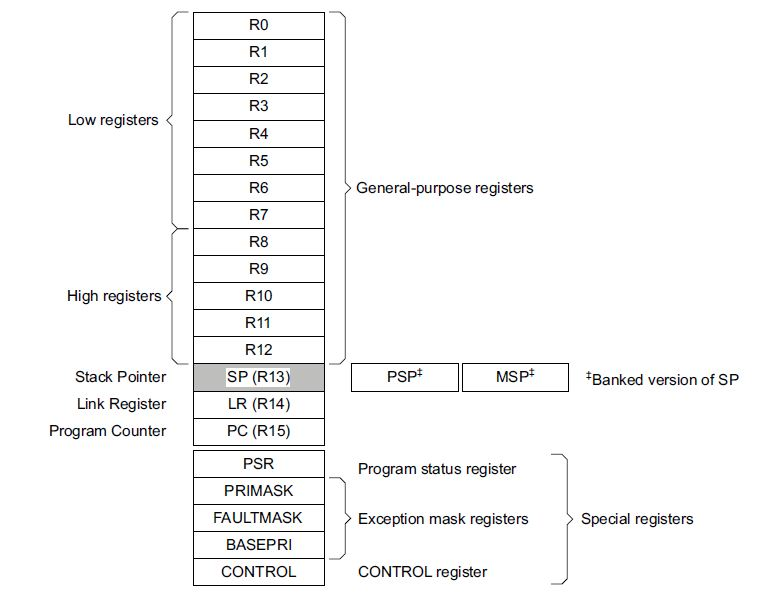
\includegraphics[width=5in]{figure/CM3_Registers}}
\caption[Cortex-M3 Registers] {Cortex-M3 Registers\cite{nxp.lpc17xx.manual}}
\label{fig_cm3_registers}
\end{figure}

\begin{itemize}
\item R0-R12 are 32-bit general purpose registers for data operations. Some 16-bit Thumb instructions can only access the low registers (R0-R7).

\item R13(SP) is the stack pointer alias for two banked registers shown as follows: 
    \begin{itemize}
    \item {\em Main Stack Pointer (MSP)}: This is the default stack pointer 
    and also reset value. It is used by the OS kernel and exception handlers. 
    \item {\em Process Stack Pointer (PSP)}: 
    This is used by user application code.
    \end{itemize}
On reset, the processor loads the MSP with the value from address 0x00000000.
The lowest 2 bits of the stack pointers are always 0, which means they are always word aligned.

In Thread mode, when bit$[1]$ of the CONTROL register is 0, MSP is used. When bit$[1]$ of the CONTROL register is 1, PSP is used.
\item R14(LR) is the link register. The return address of a subroutine 
      is stored in the link register when the subroutine is called. 

\item R15(PC) is the program counter. It can be written to control the program flow.
\item Special Registers are as follows:
    \begin{itemize}
    \item Program Status registers (PSRs)
    \item Interrupt Mask registers (PRIMASK, FAULTMASK, and BASEPRI)
    \item Control register (CONTROL)
    \end{itemize}

\end{itemize}
When at privilege level, all the registers are accessible. When at unprivileged (user) level, access to these registers are limited. 

\subsection{Processor mode and privilege levels}
\label{sec_op_mode}
The Cortex-M3 processor supports two modes of operation, Thread mode and Handler mode. 
\begin{itemize}
\item Thread mode is entered upon Reset and is used to execute application software.
\item Handler mode is used to handle exceptions. The processor returns to Thread mode when it has finished exception handling.  
\end{itemize}
Software execution has two access levels, 
Privileged level and Unprivileged (User) level. 
\begin{itemize}
\item Privileged \\
        The software can use all instructions and has access to all resources. Your RTOS kernel functions are running in this mode. 
\item Unprivileged (User) \\
        The software has limited access to {\bf $\mathtt{MSR}$} and {\bf $\mathtt{MRS}$} instructions and cannot use the {\bf $\mathtt{CPS}$} instruction.  There is no access to the system timer, NVIC , or system control block. The software might also have restricted access to memory or peripherals. User processes such as the wall clock process should run at this level.  
\end{itemize}

When the processor is in Handler mode, it is at the privileged level. When the processor is in Thread mode, it can run at privileged or unprivileged (user) level. The bit$[0]$ in CONTROL register determines the execution privilege level in Thread mode. When this bit is 0 (default), it  is privileged level when in Thread mode. When this bit is 1, it is unprivileged when in Thread mode.Figure \ref{fig_cm3_op_modes} illustrate the mode and privilege level of the processor. 
\begin{figure}[ht]
\centerline{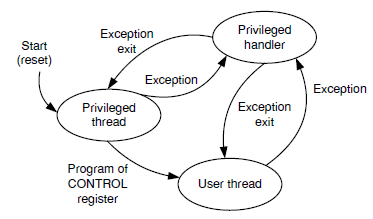
\includegraphics[width=3in]{figure/CM3_Op_Modes}}
\caption[Cortex-M3 Operating Mode and Privilege Level] {Cortex-M3 Operating Mode and Privilege Level\cite{yiu2009definitive}}
\label{fig_cm3_op_modes}
\end{figure}

Note that only privileged software can write to the CONTROL register to change the privilege level for software execution in Thread mode. Unprivileged software can use the $\mathtt{SVC}$ instruction to make a supervisor call to transfer control to privileged software. 
%You may think the $\mathtt{SVC}$ is similar as the $\mathtt{TRAP}$ for the ColdFire processor.
%The $\mathtt{SVC}$ is for generating system functions. Instead of allowing user programs to directly access hardware and kernel sensitive data, your OS may provide access to kernel through an $\mathtt{SVC}$.  
When we are in the privileged thread mode, we can directly set the control register to change to unprivileged thread mode. We also can change to unprivileged thread mode by calling $\mathtt{SVC}$ to raise an exception first  and then inside the exception handler we set the privilege level to unprivileged by setting the control register. Then we modify the $\mathtt{EXC\_RETURN}$ value in the LR (R14) to indicate the mode and stack when returning from an exception. This mechanism is often used by the kernel in its intialization phase and also context switching between privileged processes and unprivileged processes.
\subsection{Stacks}
\label{sec_stacks}
The processor uses a full descending stack. This means the stack pointer indicates the last stacked item on the stack memory. When the processor pushes a new item onto the stack, it decrements the stack pointer and then writes the item to the new memory location. 

The processor implements two stacks, the {\em main stack} and the {\em process stack}. 
One of these two stacks is banked out depending on the stack in use. This means only one stack is visible at a time as R13. 
In Handler mode, the main stack is always used. The bit$[1]$ in CONTROL register reads as zero and ignores writes in Handler mode. 
In Thread mode, the bit$[1]$ setting in CONTROL register determines whether
the main stack or the process stack is currently used. 
Table \ref{tb_cm3_mode} summarizes the processor mode, execution privilege level, and stack use options.
\begin{table}[ht]
\begin{center}
\footnotesize{
\begin{tabular}{llllll}
\hline
Processor & Used to & Privilege level for & 
\multicolumn{2}{c}{CONTROL}  & Stack used \\ 
mode      & execute & software execution  & Bit$[0]$ & Bit$[1]$\\ \hline
Thread    & Applications & Privileged   & 0  & 0 & Main Stack \\
          &              & Privileged   & 0  & 1 & Process Stack \\ 
          &              & Unprivileged & 1  & 1 & Process Stack \\ \hline
Handler   &Exception handlers & Privileged & - & 0 & Main Stack \\ \hline
\end{tabular}
}
\caption{Summary of processor mode, execution privilege level, and stack use options}
\label{tb_cm3_mode}
\end{center}
\end{table}



%LPC 1768 MCU

% memory map
\section{Memory Map}
The Cortex-M3 processor has a single fixed 4GB address space.  
Table \ref{tb_lpc1768_mem} shows how this space is used on the LPC1768.
\begin{table}[ht]
\begin{center}
\footnotesize{
\begin{tabular} {llll}
\\ \hline
Address Range & General Use & Address range details & Description \\ 
\hline \hline
$\mathtt{0x0000~0000}$ to & On-chip non-volatile  
    & $\mathtt{0x0000~0000 - 0x0007~FFFF}$ & 512 KB flash memory \\ 

$\mathtt{0x1FFF~FFFF}$    & memory \\
                 & On-chip SRAM & $\mathtt{0x1000~0000 - 0x1000~7FFF}$ 
                 & 32 KB local SRAM \\
                 & Boot ROM & $\mathtt{0x1FFF~0000 - 0x1FFF~1FFF}$
                 & 8 KB Boot ROM\\ 
\hline
$\mathtt{0x2000~0000}$ to & On-chip SRAM
    & $\mathtt{0x2007~C000 - 0x2007~FFFF}$ & AHB SRAM - bank0 (16 KB) \\
$\mathtt{0x3FFF~FFFF}$    & (typically used for
    & $\mathtt{0x2008~0000 - 0x2008~3FFF}$ & AHB SRAM - bank1 (16 KB) \\
                          & peripheral data) \\
                          & GPIO
    & $\mathtt{0x2009~C000 - 0x2009~FFFF}$ & GPIO \\
\hline
$\mathtt{0x4000~0000}$ to & APB Peripherals
    & $\mathtt{0x4000~0000 - 0x4007~FFFF}$ & APB0 Peripherals \\
$\mathtt{0x5FFF~FFFF}$ & 
    & $\mathtt{0x4008~0000 - 0x400F~FFFF}$ & APB1 Peripherals \\
                          & AHB peripherals 
    & $\mathtt{0x5000~0000 - 0x501F~FFFF}$ & DMA Controller, Ethernet  \\
                                         &&& interface, and USB interface \\
\hline
$\mathtt{0xE000~0000}$ to & Cortex-M3 Private 
    & $\mathtt{0xE000~0000 - 0xE00F~FFFF}$ & Cortex-M3 private registers(NVIC, \\
$\mathtt{0xE00F~FFFF}$   & Peripheral Bus (PPB) && MPU and SysTick Timer et. al.) \\
\hline
\end{tabular}
\caption{LPC1768 Memory Map}
\label{tb_lpc1768_mem}
}
\end{center}
\end{table}

%\begin{table}
%\begin{center}
%    \begin{tabular}{lll}
%    \\ \hline
%    0x4010 0000 &       & Reserved \\ \hline 
%    0x4008 0000 &       & APB1 peripherals \\ \hline
%    0x4000 0000 &       & APB0 peripherals (UART0-1, TIMER0-1 et. al.) \\ \hline
%    0x2400 0000 &       & Reserved \\ \hline
%    0x2200 0000 &       & AHB SRAM bit band alias addressing \\ \hline
%    0x200A 0000 &       & Reserved \\ \hline 
%    0x2009 C000 &       & GPIO \\ \hline
%    0x2008 4000 &       & Reserved \\ \hline
%    0x2007 C000 & 32 KB & AHB SRAM (2 blocks of 16 KB) \\ \hline
%    0x1FFF 2000 &       & Reserved \\ \hline
%    0x1FFF 0000 & 8 KB  & Boot ROM \\ \hline
%    0x1000 8000 &       & Reserved \\ \hline
%    0x1000 0000 & 32 KB & Local SRAM \\ \hline 
%    0x0008 0000 &       & Reserved \\ \hline
%    0x0000 0000 & 512 KB& On-chip flash
%    \\ \hline
%    \end{tabular}
%    \caption{LPC1768 MCU Memory Map}
%    \label{tb_lpc1768_mem}
%\end{center}
%\end{table}

Note that the memory map is not continuous. For memory regions not shown in the table, they are reserved. When accessing reserved memory region, the processor's behavior is not defined. All the peripherals are memory-mapped and the LPC17xx.h file defines the data structure to access the memory-mapped peripherals in C. 

\section{Exceptions and Interrupts}
The Cortex-M3 processor supports system exceptions and interrupts. 
The processor and the Nested Vectored Interrupt Controller (NVIC) 
prioritize and handle all exceptions. The processor uses {\em Handler mode}
to handle all exceptions except for reset.

\subsection{Vector Table}
Exceptions are numbered 1-15 for system exceptions and 
16 and above for external interrupt inputs. LPC1768 NVIC supports 
35 vectored interrupts. Table \ref{tb_vector_table} shows system exceptions  
and some frequently used interrupt sources. 
See Table 50 and Table 639 in \cite{nxp.lpc17xx.manual} for the complete
exceptions and interrupts sources. 
On system reset, the vector table is fixed at address $\mathtt{0x00000000}$. 
Privileged software can write to the VTOR (within the System Control Block) to relocate the vector table start address to a different memory location, in the range $\mathtt{0x00000080}$ to $\mathtt{0x3FFFFF80}$. 


\begin{table}[ht]
\begin{center}
\footnotesize{
\begin{tabular}{llllll}
\hline
Exception & IRQ    & Vector address & Exception & Priority & C PreFix \\
number    & number & or offset      & type      &          &             \\
\hline
1  & -    & $\mathtt{0x00000004}$ & Reset & -3, the highest & \\
2  & -14  & $\mathtt{0x00000008}$ & NMI   & -2, & NMI\_\\
3  & -13  & $\mathtt{0x0000000C}$ & Hard fault & -1 & HardFault\_\\
4  & -12  & $\mathtt{0x00000010}$ & Memory & Configurable & MemManage\_\\
   &      &                       & management fault \\
$\vdots$ \\
11 & -5   & $\mathtt{0x0000002C}$ & SVCall & Configurable & SVC\_\\
$\vdots$ \\
14 & -2   & $\mathtt{0x00000038}$ & PendSV & Configurable & PendSVC\_\\
15 & -1   & $\mathtt{0x0000003C}$ & SysTick & Configurable & SysTick\_\\
16 & 0    & $\mathtt{0x00000040}$ & WDT     & Configurable & WDT\_IRQ \\
17 & 1    & $\mathtt{0x00000044}$ & Timer0  & Configurable & TIMER0\_IRQ \\
18 & 2    & $\mathtt{0x00000048}$ & Timer1  & Configurable & TIMER1\_IRQ \\
19 & 3    & $\mathtt{0x0000004C}$ & Timer2  & Configurable & TIMER2\_IRQ \\
20 & 4    & $\mathtt{0x00000050}$ & Timer3  & Configurable & TIMER3\_IRQ \\
21 & 5    & $\mathtt{0x00000054}$ & UART0   & Configurable & UART0\_IRQ \\
22 & 6    & $\mathtt{0x00000058}$ & UART1   & Configurable & UART1\_IRQ \\
23 & 7    & $\mathtt{0x0000005C}$ & UART2   & Configurable & UART2\_IRQ \\
24 & 8    & $\mathtt{0x00000060}$ & UART3   & Configurable & UART3\_IRQ \\
$\vdots$ \\
\hline
\end{tabular}
\caption{LPC1768 Exception and Interrupt Table}
\label{tb_vector_table}
}
\end{center}
\end{table}
\subsection{Exception Entry}
Exception entry occurs when there is a pending exception with sufficient priority and either
\begin{itemize}
\item the processor is in Thread mode
\item the processor is in Handler mode and the new exception is of higher priority than the exception being handled, in which case the new exception preempts the original exception (This is the nested exception case which is not required in our RTOS lab).
\end{itemize}
When an exception takes place, the following happens
%\begin{itemize}
%\item Stacking(processor automatically push eight registers' contents to stack)
%\item Vector fetch (reading the exception handler starting address from the vector table)
%\item{Update of the SP, LR and PC}
%\end{itemize}

\begin{itemize}
\item{Stacking} \\

When the processor invokes an exception (except for tail-chained or a late-arriving exception, which are not required in the RTOS lab), it automatically stores the following eight registers to the SP:
\begin{itemize}
\item R0-R3, R12
\item PC (Program Counter)
\item PSR (Processor Status Register)
\item LR (Link Register, R14)
\end{itemize}
Figure \ref{fig_cm3_stack_frame} shows the exception stack frame. 
Note that by default the stack frame is aligned to double word 
address starting from Cortex-M3 revision 2.  
The alignment feature can be turned off by programming the 
STKALIGN bit in the System Control Block (SCB) 
Configuration Control Register (CCR) to 0.
On exception entry, the processor uses bit$[9]$ of the stacked PSR
to indicate the stack alignment. On return from the exception, it uses this
stacked bit to restore the correct stack alignment.
\begin{figure}[ht]
\centerline{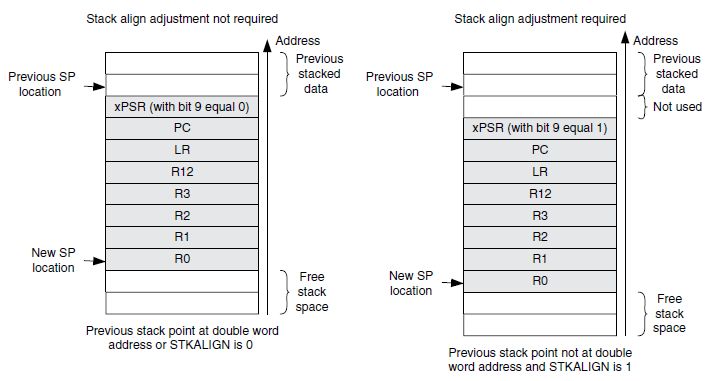
\includegraphics[width=5in]{figure/CM3_Exception_Stack_Frame}}
\caption[Cortex-M3 Exception Stack Frame] 
        {Cortex-M3 Exception Stack Frame \cite{yiu2009definitive}}
\label{fig_cm3_stack_frame}
\end{figure}

\item{Vector Fetching} \\
While the data bus is busy stacking the registers, the instruction bus fetches
the exception vector (the starting address of the exception handler) from the vector table. The stacking and vector fetch are performed on separate bus interfaces, hence they can be carried out at the same time.
\item{Register Updates} \\
After the stacking and vector fetch are completed, the exception vector
will start to execute. On entry of the exception handler, the following
registers will be updated as follows:
\begin{itemize}
    \item SP: The SP (MSP or PSP) will be updated to the new location during stacking. Stacking from the privileged/unprivileged thread to the first level of the exception handler uses the MSP/PSP. During the execution of exception handler routine, the MSP will be used when stack is accessed.
    \item PSR: The IPSR will be updated to the new exception number
    \item PC: The PC will change to the vector handler when the vector fetch completes and starts fetching instructions from the exception vector.
    \item LR: The LR will be updated to a special value called $\mathtt{EXC\_RETURN}$. This indicates which stack pointer corresponds to the stack frame and what operation mode the processor was in before the exception entry occurred.  
    \item Other NVIC registers: a number of other NVIC registers will be updated .For example the pending status of exception will be cleared and the active bit of the exception will be set.
\end{itemize}
\end{itemize}
\subsection{$\mathtt{EXC\_RETURN}$ Value}
\label{sec_exc_return}
$\mathtt{EXC\_RETURN}$ is the value loaded into the LR on exception entry. The exception mechanism relies on this value to detect when the processor has completed an exception handler. The $\mathtt{EXC\_RETURN}$ bits $[31:4]$ is always
set to $\mathtt{0xFFFF FFF}$ by the processor. When this value is loaded into the PC, it indicates to the processor that the exception is complete and the processor initiates the exception return sequence.
Table \ref{tb_exc_return_bits} describes the $\mathtt{EXC\_RETURN}$ bit fields. 
Table \ref{tb_cm3_exc_return_vals} lists Cortex-M3 allowed $\mathtt{EXC\_RETURN}$ values. 
\begin{table}[ht]
\begin{center}
\footnotesize{
\begin{tabular}{llllll}
\hline
Bits   &  31:4  & 3  & 2 &1 & 0 \\ \hline
Description & $\mathtt{0xFFFF FFF} $ &Return mode & Return stack & Reserved; & Process state \\
       &  & (Thread/Handler) & & must be 0 & (Thumb/ARM) \\ \hline
\end{tabular}
\caption[$\mathtt{EXC\_RETURN}$ bit fields]
{$\mathtt{EXC\_RETURN}$ bit fields \cite{yiu2009definitive}}
\label{tb_exc_return_bits}
}
\end{center}
\end{table}

\begin{table}[ht]
\begin{center}
\footnotesize{
\begin{tabular}{llll}
\hline
Value  & \multicolumn{3}{c}{Description} \\ \hline
       & Return  & Exception return & SP after return \\
       & Mode    & gets state from  & \\ \hline
$\mathtt{0xFFFFFFF1}$ & Handler & MSP & MSP \\
$\mathtt{0xFFFFFFF9}$ & Thread  & MSP  & MSP\\
$\mathtt{0xFFFFFFFD}$ & Thread  & PSP  & PSP \\ \hline
\end{tabular}
\caption[$\mathtt{EXC\_RETURN}$ Values on Cortex-M3]
{$\mathtt{EXC\_RETURN}$ Values on Cortex-M3}
\label{tb_cm3_exc_return_vals}
}
\end{center}
\end{table}

\subsection{Exception Return}
Exception return occurs when the processor is in Handler mode and executes one of the following instructions to load the $\mathtt{EXC\_RETURN}$ value into the PC:
\begin{itemize}
\item a $\mathtt{POP}$ instruction that includes the PC. This is normally used when the $\mathtt{EXC\_RETURN}$ in LR upon entering the exception is pushed onto the stack.  
\item a $\mathtt{BX}$ instruction with any register. This is normally used when LR contains the proper $\mathtt{EXC\_RETURN}$ value before the exception return, then $\mathtt{BX~ LR}$ instruction will cause an exception return.
\item a $\mathtt{LDR}$ or $\mathtt{LDM}$ instruction with the PC as the destination. This is another way to load PC with the $\mathtt{EXC\_RETURN}$ value.
\end{itemize}

Note unlike the ColdFire processor which has the $\mathtt{RTE}$ as the 
special instruction for exception return, in Cortex-M3, a normal return instruction is used so that the whole interrupt handler can be implemented as a C subroutine. 

When the exception return instruction is executed, the following exception return sequences happen:
\begin{itemize}
\item Unstacking: The registers (i.e. exception stack frame) pushed to the stack will be restored. The order of the POP will be the same as in stacking. The SP will also be changed back.
\item NVIC register update: The active bit of the exception will be cleared. The pending bit will be set again if the external interrupt is still asserted, causing the processor to reenter the interrupt handler.
\end{itemize}


\section{Data Types}
The processor supports 32-bit words, 16-bit halfwords and 8-bit bytes. 
It supports 64-bit data transfer instructions. 
All data memory accesses are managed as little-endian.


%\section{System Control Block}
%\section{Pin Control Block}
%\section{GPIO}

%%% Local Variables:
%%% mode: latex
%%% TeX-master: "main_book"
%%% End:
